\documentclass[titlepage,11pt]{scrartcl}
\usepackage{graphicx}
\usepackage[utf8]{inputenc}
\usepackage{amsmath}
\usepackage{amsmath}
\usepackage{amsfonts}
\usepackage{amssymb}
\usepackage{listings}
\usepackage[pdftex]{hyperref}
\usepackage[x11names,table]{xcolor}
\usepackage{graphicx}
\usepackage{float}

\title{	
    \normalfont\normalsize
	\vspace{25pt}
	{\huge Simulación\ Proyecto 1}
	\vspace{12pt}
}

\author{\LARGE Victor Manuel Cardentey Fundora C411}

\date{}

\begin{document}

\maketitle

\section{Github:}
	\url{https://github.com/Vitico99/overloaded-harbor-simulation.git}

\section{Problema:}

	\textbf{Puerto Sobrecargado (Overloaded Harbor)}

	En un puerto de supertanqueros que cuenta con 3 muelles y un remolcador para la descarga de estos barcos de manera simultánea se desea conocer el tiempo promedio de espera de los barcos para ser cargados en el puerto. El puerto cuenta con un bote remolcador disponible para asistir a los tanqueros. Los tanqueros de cualquier tamaño necesitan de un remolcador para aproximarse al muelle desde el puerto y para dejar el muelle de vuelta al puerto. El tiempo de intervalo de arribo de cada barco distribuye mediante una función exponencial con $\lambda = 8$ horas. Existen tres tamaños distintos de tanqueros: pequeño, mediano y grande, la probabilidad correspondiente al tamaño de cada tanquero se describe en la tabla siguiente. El tiempo de carga de cada tanquero depende de su tamaño y los parámetros de distribución normal que lo representa también se describen en la tabla siguiente.

	\begin{center}
		\begin{tabular}
			{c c c}
			\rule[-1ex]{0pt}{1.5ex} Tamaño & Probabilidad de Arribo & Tiempo de Carga \\
			\rule[-1ex]{0pt}{1.5ex} Pequeño & 0.25 & $\mu = 9, \sigma^2 = 1$ \\
			\rule[-1ex]{0pt}{1.5ex} Mediano & 0.25 & $\mu = 12, \sigma^2 = 2$ \\
			\rule[-1ex]{0pt}{1.5ex} Grande & 0.5 & $\mu = 18, \sigma^2 = 3$ \\
		\end{tabular}
	\end{center}

	De manera general, cuando un tanquero llega al puerto, espera en una cola (virtual) hasta que exista un muelle vacío y que un remolcador esté disponible para atenderle. Cuando el remolcador está disponible lo asiste para que pueda comenzar su carga, este proceso demora un tiempo que distribuye exponencial con $\lambda = 2$ horas. El proceso de carga comienza inmediatamente después de que el barco llega al muelle. Una vez terminado este proceso es necesaria la asistencia del remolcador (esperando hasta que esté disponible) para llevarlo de vuelta al puerto, el tiempo de esta operación distribuye de manera exponencial con $\lambda = 1$ hora. El traslado entre el puerto y un muelle por el remolcador sin tanquero distribuye exponencial con $\lambda = 15$ minutos. Cuando el remolcador termina la operación de aproximar un tanquero al muelle, entonces lleva al puerto al primer barco que esperaba por salir, en caso de que no exista barco por salir y algún muelle esté vacío, entonces el remolcador se dirige hacia el puerto para llevar al primer barco en espera hacia el muelle vacío; en caso de que no espere ningún barco, entonces el remolcador esperará por algún barco en un muelle para llevarlo al puerto. 
	
	Cuando el remolcador termina la operación de llevar algún barco al puerto, este inmediatamente lleva al primer barco esperando hacia el muelle vacío. En caso de que no haya barcos en los muelles, ni barcos en espera para ir al muelle, entonces el remolcador se queda en el puerto esperando por algún barco para llevar a un muelle. 
	
	Simule completamente el funcionamiento del puerto. Determine el tiempo promedio de espera en los muelles.

\section{Principales ideas de la soluci\'on:}

    Se utiliz\'o un modelo de simulaci\'on basado en eventos discretos.
    Durante el proceso de simulaci\'on generamos los eventos que conforman la l\'inea temporal de la simulaci\'on,
    determinamos el evento m\'as pr\'oximo dentro de la l\'inea temporal y actualizamos las variables de la simulaci\'on de acuerdo al tipo de evento ocurrido.\\
    Para este problema definimos cuatro eventos:
	
	\begin{enumerate}
		\item Arribo de un supertanquero al puerto
		\item Arribo de un remolcador al muelle
		\item Partida de un remolcador desde el muelle
		\item Arribo de un remolcador al puerto
	\end{enumerate}

    Durante la ocurrencia de cada uno de estos eventos se pueden agregar nuevas ocurrencias de eventos dentro de la l\'inea temporal.\\
    Optamos por definir los eventos en dependencia de los remolcadores en lugar de los supertanqueros debido a que los remolcadores pueden realizar acciones incluso
    durante la total ausencia de los supertanqueros en el sistema (p.e. desplazarse hacia el puerto para esperar la llegada de barcos) pero los supertanqueros solo pueden modificar el comportamiento del
    sistema con la asistencia de los remolcadores.\\
    Debido a que se implementar\'a un modelo generalizado del problema para simular la l\'inea temporal utilizaremos una cola de prioridad
    para almacenar los eventos y poder obtener el pr\'oximo evento (m\'inimo) de forma eficiente. Las colas del puerto y del muelle se asumen cumplen el principio FIFO y que los par\'ametros de
    las variables aleatorias que intervienen en la soluci\'on est\'an expresadas en horas, para la simulaci\'on de las variables aleatorias utilizaremos la funcion \text{random.random} de Python.


\section{Descripci\'on del Modelo:}

	\begin{enumerate}
		\item \textbf{Variables de tiempo:}
			\begin{itemize}
				\item $t$: Tiempo actual dentro de la simulaci\'on.
				\item $T$: Duraci\'on total de la simulaci\'on.
			\end{itemize}
		\item \textbf{Variables contadoras:}
			\begin{itemize}
				\item $N\_arrived\_port$: Cantidad de arribos de supertanqueros al puerto
				\item $N\_arrived\_dock$: Cantidad de arribos de supertanqueros a los muelles
				\item $N\_departed\_dock$: Cantidad de supertanqueros que han partido desde los muelles hacia el puerto
				\item $N\_departed\_port$: Cantidad de supertanqueros que han partido desde el puerto
			\end{itemize}
		\item \textbf{Variables de estado:}
			\begin{itemize}
				\item $port\_queue$: Cola de barcos esperando en el puerto con destino al muelle
				\item $dock\_queue$: Cola de barcos esperando en los muelles con destino al puerto
				\item $docks$: Asocia cada muelle con el supertanquero que est\'a realizando una operaci\'on en dicho muelle, de no encontrarse ning\'un supertanquero en un muelle su valor ser\'a 0
				\item $tugboats$: Asocia cada remolcador con el supertanquero al que est\'a asistiendo. En caso de no estar asistiendo a ning\'un supertanquero su valor es 0
				\item $tugboats_loc$: Asocia cada remolcador con su localizaci\'on actual, puede ser muelle o puerto, dado que esta informaci\'on es relevante para el c\'alculo de tiempos y determinar el comportamiento de los remolcadores
				\item $ship_type$: Asocia cada supertanquero con su tipo
            \end{itemize}
		\item \textbf{Variables de salida:}
			\begin{itemize}
                \item $arrived\_port$: Tiempos de los arribos de supertanqueros al puerto
				\item $arrived\_dock$: Tiempos de los arribos de supertanqueros a los muelles
				\item $departed\_dock$: Tiempos de las partidas de los supertanqueros desde el muelle
				\item $departed\_port$: Tiempos de las partidas de los supertanqueros desde el puerto
			\end{itemize}

        \item \textbf{Lista de Estados:}
			\begin{itemize}
                \item $t\_next\_arrive$: Tiempo del pr\'oximo arribo de un supertanquero
				\item $t\_arrive\_dock$: Tiempos de los arribos de remolcadores a los muelles
				\item $t\_depart\_dock$: Tiempos de las partidas de remolcadores desde los muelles
				\item $t\_depart\_port$: Tiempos de las llegadas de remolcadores al puerto
			\end{itemize}
        
        \item \textbf{Inicializaci\'on:}
			\begin{itemize}
                \item $t = N\_arrived\_port = N\_arrived\_dock = N\_departed\_dock = N\_departed\_port = 0$
				\item $port\_queue = dock\_queue = t\_arrive\_dock = t\_depart\_dock = t\_depart\_port  = \emptyset$
				\item $docks = [0...0_{k_1}]$
				\item $tugboats = [0...0_{k_2}]$
                \item $t\_next\_arrive = exp(\lambda)$
			\end{itemize}
        
        \item \textbf{Caso 1: $\min(t\_next\_arrive, t\_arrive\_dock, t\_depart\_dock, t\_depart\_port)  == t\_next\_arrive$}
			\begin{itemize}
                \item $t = t\_next\_arrive$ 
                \item Genera el nuevo evento de arribo $t\_next\_arrive += exp(\lambda)$
                \item $N\_arrived\_port = N\_arrived\_port + 1$ y registrar en $arrived\_port$
				\item Si $\exists 0 \in docks \land \exists 0 \in tugboats \land port\_queue = \emptyset$ genera un nuevo evento en $t\_arrive\_dock$
				\item En otro caso agregar el barco a la cola del puerto $port\_queue$ 
			\end{itemize}
        
        \item \textbf{Caso 2: $\min(t\_next\_arrive, t\_arrive\_dock, t\_depart\_dock, t\_depart\_port)  == \min(t\_arrive\_dock)$}
			\begin{itemize}
                \item $t = \min(t\_arrive\_dock)$
                \item $N\_arrived\_dock = N\_arrived\_dock + 1$ y registrar en $arrived\_dock$
                \item Si el remolcador tra\'ia un barco, supongamos el remolcador $i$, si $tugboats[i] \neq 0$ calcular el tiempo de descarga y generar un nuevo evento en $t\_depart\_dock$
                \item Reasignar al remolcador $i$, el cual puede llevar un barco al puerto o ir al puerto a esperar (genera evento en $t\_depart\_port$), traer un barco del puerto (genera evento en $t\_arrive\_dock$) o quedarse esperando en el puerto (no se generan eventos)   
			\end{itemize}

        \item \textbf{Caso 3: $\min(t\_next\_arrive, t\_arrive\_dock, t\_depart\_dock, t\_depart\_port)  == \min(t\_depart\_dock)$}
			\begin{itemize}
                \item $t = \min(t\_depart\_dock)$
                \item $N\_departed\_dock = N\_departed\_dock + 1$ y registrar en $departed\_dock$
                \item Si $\exists 0 \in tugboats$ a\~nadir un evento en $t\_depart\_port$
                \item En otro caso agreagar el barco a la cola de los muelles $dock\_queue$  
			\end{itemize}
        
        \item \textbf{Caso 4: $\min(t\_next\_arrive, t\_arrive\_dock, t\_depart\_dock, t\_depart\_port)  == \min(t\_depart\_port)$}
			\begin{itemize}
                \item $t = \min(t\_depart\_port)$
                \item Si $tugboats[i] \neq 0$ entonces $N\_departed\_port = N\_departed\_port + 1$ y registrar en $departed\_port$
                \item Reasignar el remolcador $i$ 
			\end{itemize}
	\end{enumerate}



\section{Consideraciones obtenidas:}

	Luego de correr 20 simulaciones por un per\'iodo de tiempo de un a\~no, llegamos a un resultado de 26.038 hrs como
	promedio de tiempo de espera, sin embargo, estos resultados, debido al car\'acter aleatorio de la simulaci\'on, variaban con cada ejecuci\'on.
	Por tanto ejecutamos simulaciones para todos posibles per\'iodos de d\'ias hasta un m\'aximo de un a\~no, a trav\'es de estas 
	simulaciones obtuvimos la siguiente gr\'afica en la cual podemos observar un comportamiento creciente cuando la cantidad de d\'ias simulados 
	es peque\~na y luego una estabilizaci\'on donde los valores de las simulaciones para $T >= 100$ se encuentran en el rango $[26,28]$ por lo cual el promedio del tiempo de espera ser\'ia $\approx 27$.
	
	\begin{figure}[htb]
		\begin{center}
			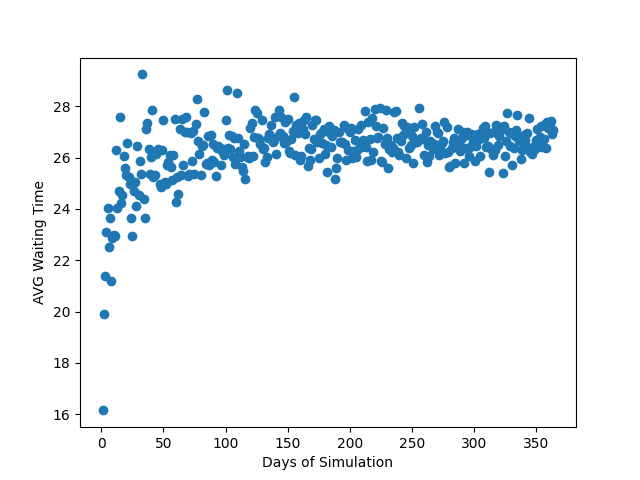
\includegraphics[width=\columnwidth]{./g.png}
		\end{center}
		\caption{Gr\'afica 3 muelles y 1 remolcador}
	\end{figure}

	Tambi\'en se utiliz\'o el modelo para comprobar que aumentar la cantidad de remolcadores disminuye el promedio del tiempo de espera, tener un remolcador por muelle redujo el promedio de espera para $T >= 100$ a $\approx 23$. Adem\'as se comprob\'o que tener m\'as remolcadores que
	muelles reporta bastante poco beneficio por lo que si se tiene una misma cantida de remolcadores y de muelles ser\'ia mejor incrementar la cantidad de muelles para mejorar la eficiencia.

	\begin{figure}[htb]
		\begin{center}
			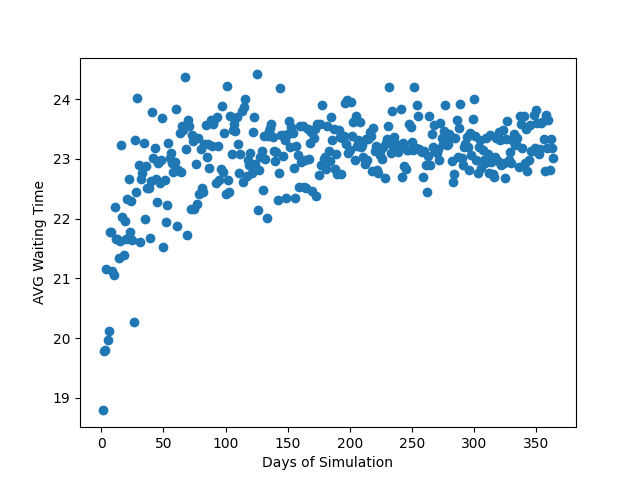
\includegraphics[width=\columnwidth]{./g1.png}
		\end{center}
		\caption{Gr\'afica 3 muelles y 3 remolcadores}
	\end{figure}

	\begin{figure}[htb]
		\begin{center}
			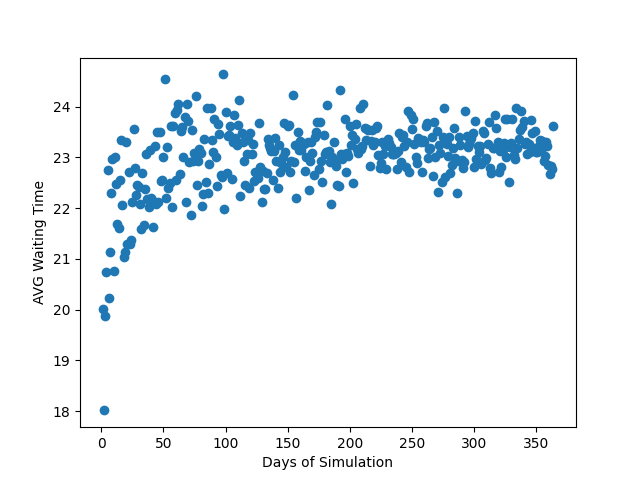
\includegraphics[width=\columnwidth]{./g2.png}
		\end{center}
		\caption{Gr\'afica 3 muelles y 5 remolcadores}
	\end{figure}
	
\end{document}
